% UONTEST.TEX - a sample file for the UONTHESIS document style.
% revised by Colin Johnson (Colin.Johnson@nottingham.ac.uk), 2020-02-18
%
\documentclass[11pt]{uonthesis}

\usepackage[titletoc]{appendix}
\usepackage{graphicx, multirow, multirow, subcaption, amsmath, array} % put additional packages here
\usepackage{algorithm, algpseudocode}
\newcolumntype{P}[1]{>{\centering\arraybackslash}p{#1}}
%\usepackage[backend=biber, sorting=nyt, style=numeric, firstinits=true]{biblatex}
\bibliographystyle{unsrt} 
%\addbibresource{refs.bib}

\renewcommand{\appendixtocname}{List of appendices}

\title{Real-time prediction of lane-level traffic speeds using Mixed Deep Learning model with Apache Spark and Kafka}
\author{Makoto Ono}
\prevdegrees{MSc}
\university{The University of Nottingham}
\degree{MSc Computer Science with Artificial Intelligence}
\date{September 2024}

%%%%%%%%%%%%%%%%%%%%%%%%%%%%%%%%%%%%%%%%%%%%%%%%%%%%%%%%%%%%%%%%%%%%%%%%%%%%%%%%%%%%
\begin{document}

\begin{frontmatter}
\maketitle
\tableofcontents

\begin{abstract}
In the era of rapid urbanisation and the ever-increasing car ownership in the world, traffic congestions have been affecting the daily lives of major cities. Road traffic state prediction can alleviate this issue together with the development of other intelligent traffic systems and autonomous vehicles, and the prediction of lane-level traffic speeds plays a vital role for the design and implementation of these systems, aiding vehicles to make informed decisions for driving on the road. In order to bridge the gap between the ever-changing traffic state and the prediction model, real-time prediction of lane-level traffic speeds is essential. However, processing the massive volume of trajectory data of all vehicles on the road requires high computational power. With the help of scalable and low-latency big data processing of Apache Spark and Kafka, this paper proposes a real-time data processing and prediction method for lane-level traffic speed using a deep learning model called Mixed Deep Learning model. The model was trained on the Next Generation Simulation (NGSIM) dataset, which contains detailed vehicle trajectory data of a section of Highway US-101 in Los Angeles, California. In the proposed method, the data is streamed using a distributed streaming platform called Kafka into Apache Spark, a big data processing platform, in which the model was integrated and makes real-time prediction. The results of our experiments show that the model is able to predict the lane-level traffic speeds of several seconds ahead in real-time in our computational laboratory setting. The proposed method can be integrated into the existing systems and utilised to improve the efficiency of road traffic and relieve traffic congestions, leading to a positive impact on the environment and the society.
% ADD KEYWORDS
\end{abstract}

\begin{acknowledgements}
I would like to thank the following people and organisation, without whom I would not have been able to complete this research and my master's degree:\\ 
\noindent My supervisor, Rebecca Tickle for her guidance and strong support throughout the project\\
\noindent The U.S. Department of Transportation Federal Highway Administration for making their dataset publicly available\\
\noindent My honourable coursemates: Raonak, Kamal, Nary and Emily, with whom I sat in the C11 Computer Room all day during the course, for their encouragement and support\\
\noindent Last but not least, my family for their love and support throughout my life

\end{acknowledgements}

\end{frontmatter}

%%%%%%%%%%%%%%%%%%%%%%%%%%%%%%%%%%%%%%%%%%%%%%%%%%%%%%%%%%%%%%%%%%%%%%%%%%%%%%%%%%%%
\chapter{Introduction}

\section{Introduction and Motivation}
Nowadays, urban transportation across the globe is facing unprecedented challenges: traffic congestion, road safety, pollution, and so on, due to rapid urbanisation and a rapid increase in car ownership and traffic volume in the last several decades \cite{congestion1}\cite{congestion2}. In addressing these problems, smart city and autonomous vehicles are of a particular interest of some researchers and policy makers, recently, and vehicle trajectory analysis, modelling, prediction play an essential role for realising these concepts. The efforts have been made so far in the name of development of Intelligent Transportation Systems (ITS) \cite{ITS} and, together with the evolution of Advanced Driver-Assistance Systems (ADAS) and Autonomous Vehicles (AVs), they have contributed to the improved efficiency of transportation systems, reduction of traffic congestion, and enhancement of road safety \cite{adas}. In the future, the integration of these technologies will make it possible to implement large-scale real-time vehicle information sharing and processing. 

% Collection of traffic data: road sensor, GPS, video calibration, etc.
Traffic data can be collected from various sources such as road sensors, video cameras \cite{ngsim}, and GPS devices \cite{Zhang20231124}. Such traffic data can be used to analyse traffic patterns \cite{trafficpattern} and predict traffic congestion \cite{GOMES2023200268}. However, the analysis and exploitation of traffic flow data poses several challenges, such as the large volume of data, the complexity of the data, and the need for real-time processing. In order to address these challenges, researchers have made a number of attempts to extract traffic flow information from various data sources, as described in details in Chapter 2.

% Traffic speed prediction: macro-to-microscopic including city-level, regional-level, road-level, lane-level  
When it comes to traffic state analysis, we have to consider the scope of the analysis. Traffic prediction can be performed at different levels of granularity, ranging from city-level to lane-level. City-level traffic prediction aims to predict hotspots of urban-scale traffic events such as congestions \cite{macnnimage} and accidents \cite{Zhou_Wang_Xie_Chen_Liu_2020}, while road-level traffic speed prediction aims to predict the average speed of traffic on a specific road \cite{Sigurdsson2018RoadTC}. Lane-level traffic speed prediction aims to predict the speed of traffic in a specific lane of a road \cite{gcn1}\cite{gcn2}. Lane-level traffic state forecasting is becoming an important topic of Intelligent Vehicle Infrastructure Cooperative Systems (IVICS) which is a new development of ITS, because the short-term traffic states of lanes in a road section differ in traffic speed, volume and occupancy, and the optimised use of all lanes help mitigate traffic congestions \cite{GU20191}. Moreover, the lane-level traffic state prediction can aid individual drivers to make informed decisions on the road, making them aware of traffic condition ahead of them in more details.

However, Lane-level traffic speed prediction is particularly challenging because it requires the prediction of the speed of individual vehicles in a specific lane, which can be affected by a variety of factors such as the number of lanes, the presence of on and off ramps, and the behaviour of other vehicles.

In order to address these factors, in recent years, deep learning methods such as Recurrent Neural Networks (RNNs) which includes Long Short Term Memory networks, and Graph Neural Networks (GNNs) have been widely used for lane-level traffic state prediction, as the work of Li et al. \cite{li2024unifyinglaneleveltrafficprediction} has shown performance of a number of different models. According to the paper, those involving 
convolution or graph neural networks have been shown to be effective in capturing the spatial and temporal dependencies in vehicle trajectory data.

Applying such traffic flow prediction models to real-world road environment requires the models to be able to process the large volume of data generated by vehicles on the road in real-time. The real-time processing of traffic flow and vehicle trajectory data poses another challenge: the constant stream of spatial data with high dimensionality, typically generated by road sensors or GPS, adds more complexity to trajectory data analysis and traffic prediction in terms of its scalability. Some researchers \cite{Sigurdsson2018RoadTC}\cite{9077707}\cite{Yang2019} have tried to address this challenge by leveraging distributed computing systems' scalability and low-latency to process a stream of traffic data in real-time.

\section{Aims and Objectives}
To our knowledge, however, the existing works have not yet provided a comprehensive solution to the real-time prediction of lane-level traffic speeds using a deep learning model. The objectives of this study are: (1) to provide the comprehensive overview of the existing dataset which are suitable for lane-level traffic speed prediction, (2) to provide a real-time prediction method using a Mixed Deep Learning model with Apache Spark and Kafka with a thorough description of model implementation, (3) to evaluate the performance of the proposed method using the Next Generation Simulation (NGSIM) dataset, (4) to examine the feasibility of short-term prediction of traffic flow state in real-time and the applicability of the proposed method to the real-world road environment.

In the next chapter, we provide a literature review of the existing works in the field of lane-level traffic speed prediction. Chapter 3 introduces the methodology including the dataset, the distributed data processing platforms and the deep learning model used for this study, the real-time prediction framework, and the evaluation metrics. In Chapter 4, we present the results of the experiments and analyse them. In Chapter 5, the limitations of our study results and suggestions for future work are discussed. Finally, the conclusion of the study is provided in Chapter 6.

\chapter{Literature Review}

\section{Research Field Challenges}
When performing lane-level traffic state prediction, researchers are required to address common challenges. The most relevant ones can fall into the following categories:

\begin{itemize}
    \item Scarcity of highly detailed, granular traffic datasets:
The datasets are oftentimes difficult to collect because traffic flow is a wide-ranging spatiotemporal phenomenon, and it is very challenging to collect continuous data from such wide-ranging domain \cite{seo2020evaluation}. For example, usual loop detectors only collect data at a specific point, and combining data in other formats (data fusion) (i.e., Object tracking data from CCTV footage) can be a tough challenge. Consequently, there are only a few datasets available that distinguish traffic between individual lanes, which makes it difficult to train and evaluate lane-level traffic prediction models.
    \item Anomaly and complexity of urban traffic environment:
Urban road environment has lots of variables such as not only traffic accidents, events, weather, but also Vehicle to Infrastructure interaction, Vehicle to Vehicle interaction, multimodality, generalizability (robustness to real-world road environment), etc. and they make the task of vehicle trajectory analysis more complex. The effort applying modern deep learning methods such as Long Short Time Memory networks and Generative Adversarial Networks (GANs) \cite{rossi2021vehicle}, have been made to improve the prediction model accuracy. Especially in microscopic road traffic analysis of multi-lane dual carriageways, complexity of multi-lane, multi-class traffic introduces additional challenges due to the uncertainty in human behaviours, such as lane changing \cite{DAHIYA2022100066}.
    \item Scalability and real-time processing:
The real-time processing of vehicle trajectory data is a challenging task due to the large volume of data with high dimensionality generated by vehicles on the road. The data must be processed in real-time in order to provide accurate predictions of traffic speeds. The use of distributed computing systems can help to address this challenge by providing a scalable and low-latency platform for processing vehicle trajectory data in real-time.  % add more references
\end{itemize}

\section{Suitable Datasets for Lane-level Traffic Prediction}
As explained in the previous section, the scarcity of datasets is one of the major challenges in the field of lane-level traffic prediction. However, apart from NGSIM dataset which is used in this study and is explained in details below in this paper, there are a few more works that have been done to collect lane-level traffic data which can be exploited for the task. 

HighD dataset \cite{highDdataset} is a comprehensive collection of real vehicle trajectories captured on German autobahn by using drone footage during 2017 and 2018. The dataset contains 16.5 hours of vehicle trajectories from six different locations, which translates to 110,000 vehicles. The trajectories were extracted from high resolution footage and with a state-of-the-art computer vision algorithm: U-Net Convolutional Neural Network architecture. This achieved the resulting mean positional errors of the vehicle midpoint in longitudinal and lateral directions are below 3 cm each compared to the manually annotated ground truth. The dataset is unique in that it contains a large number of vehicles and a high level of detail, including the vehicle type, the vehicle speed, and the vehicle acceleration. However, the work is focused to capture lane-changing behaviours and the dataset only contains a small portion of datapoints with traffic congestion, which makes it unsuitable for this particular study.

Zen Traffic dataset\footnote{https://zen-traffic-data.net/english/} is a large-scale dataset of vehicle trajectories collected by Hanshin Expressway Co., Ltd. in Japan. The dataset consists of vehicle trajectories observed in five different sections of the Hanshin Expressway in Osaka, Japan, and each 2km-long section contained approximately 3,600 vehicles within the one-hour-long time frame, which makes it one of the most detailed and extensive vehicle trajectory datasets available. The data were extracted from video footage recorded on 38 cameras installed along the expressway by using a deep neural network. The dataset achieved a satisfactory level of accuracy with RMSE of 1.05m in terms of vehicle positions \cite{seo2020evaluation}. It also captured different traffic dynamics such as traffic build-ups and congestions. The dataset is publicly available for free of charge. However, for the simplicity of data preprocessing in this study we did not use this dataset as the observed sections contain curves.

\begin{figure}[ht!]
    \centering
    \includegraphics[width=14cm]{{images/pems.png}}
    \caption{The distribution of PeMS sensors in California Bay Area. The sensors are relatively scattered across the road network. From Lu et al. \protect\cite{sttrafficnet}}
    \label{fig:pems}
\end{figure}

PeMS dataset\footnote{https://pems.dot.ca.gov/} is a large-scale road traffic sensor dataset collected by the California Department of Transportation (Caltrans) and the University of California, Berkeley. The dataset contains real-time traffic data collected from over 39,000 sensors deployed on the California State Highway System. The data includes traffic flow, speed, and occupancy data of each lane collected at 30 seconds intervals, as well as incident records, lane closures, and so on. The dataset is different from the above two dataset in that it is collected by road sensors, and the sensors are relatively scattered across the road network as Fig. \ref{fig:pems} shows. Moreover, the dataset exhibits some degree of data missingness due to temporalily unoperational sensors. From these limitations, the extensive dataset is not particularly suitable for this particular study which aims to predict more detailed, short-termed lane-level traffic state, although one may find its utility in their study.

\section{Statistical and Machine Learning Approach}

One of the classical approaches to traffic state prediction is the use of statistical models. The approach includes application of Kalman filters \cite{kalman} and traffic flow theory \cite{traffictheory} to the modelling. Additionally, the Autoregressive Integrated Moving Average (ARIMA) model is widely used for time series forecasting, and it has also been applied to traffic speed prediction. The previous works \cite{karima}\cite{arimax}\cite{starima} have proved that ARIMA and its variants can predict traffic flow with high accuracy, especially at road level. However, these statistical model only consider the temporal dependency of the traffic state, which makes it difficult to capture the spatial dependencies of lane-level traffic state. Moreover, in their multi-step prediction task, each prediction is made based on the previous prediction, which makes the models prone to accumulation of prediction errors \cite{gdl}.

The effort of applying machine learning methods to traffic state prediction has also been made in the field, and such efforts include the use of Support Vector Regression \cite{svr}, XGBoost \cite{xgboost}, and K-nearest neighbour \cite{knn}. These models have been shown to be effective in capturing the temporal and spatial dependencies as they can allow data containing both dependencies as an input. However, the models are limited in terms of the complexity and amount of the data they can handle, since they still require training and prediction of each study point individually, which results in a linear increase in computational cost.

\section{Deep Learning Approach}

In order to overcome the aforementioned limitations of traditional approaches, application of deep learning to the traffic prediction has been actively explored in the recent years. Ma et al. first introduced the use of Long Short-Term Memory (LSTM) networks, which is an extension of recurrent neural networks (RNN), for long-term traffic speed prediction \cite{ma2015lstm}. Rui et al. studied the use of Gated Recurrent Unit (GRU) networks, which is another variant of RNN, for short-term traffic flow prediction \cite{rui2017gru}. The LSTM and GRU networks have been shown to be effective in capturing the temporal dependencies of traffic data, and they have been widely used for traffic speed prediction. However, RNN-based models lacks the ability to capture the spatial dependencies of traffic flow data, which makes the models underperform at lane-level traffic flow prediction. 

Addressing these disadvantages of RNN-based models, the use of Convolutional Neural Networks (CNN) are widely explored in the recent literature \cite{macnnimage}\cite{cnnzhang}. The CNN-based models is capable of spatial feature extraction, since it considers the road network or a section of the road as an image-like grid structure data. Motivated by the Shi et al.'s work \cite{convlstm}, in which the researchers integrated CNN and LSTM in one end-to-end deep learning structure, Ke et al. \cite{FCL} enhanced CNN application to taxi demand prediction or more broadly spatio-temporal prediction by proposing a model named FCL-Net which consists of multiple Conv-LSTM, LSTM, and convolutional layers. Such hybrid models including Lu et al.'s work, which this study is based on, allow a more comprehensive extraction of lane-level traffic flow dynamics, particularly in capturing the relationships between time and space. However, the complexity of the model tends to lead to high computational cost.

Some researchers have also explored Graph-based deep learning models to effectively capture the spatial patterns of the non-Euclidean input data (e.g. spatial network). Among these models, Graph Convolutional Networks (GCN) based models \cite{gcn1}\cite{gcn2}\cite{agafonov} are the most popular in this field. However, Graph Neural Network-based models may not be as directly effective in handling time dependencies as specialised time series models and may still require high expertise and computational resources in constructing and training GNN models \cite{li2024unifyinglaneleveltrafficprediction}.  

\section{Real-time Traffic Data Processing}

Regarding real-time traffic data processing framework, a number of studies have been conducted to explore the applicability of distributed data processing techniques to the traffic data processing. One of the most popular methods is to integrate Apache Kafka and Apache Spark to the real-time data preprocessing. The work of Anveshrithaa and Lavanya \cite{9077707} developed a real-time data stream processing model for forecasting vehicle traffic, using Apache Kafka and Spark for parallel processing and Long Short-Term Memory (LSTM) networks to learn the temporal features of the input traffic flow data. However, the study did not consider spatial dependencies of the input data. In addition, the study lacks a thorough explanation of the model implementation and evaluation of throughput and latency of the model.

Similarly to Anveshrithaa and Lavanya's work, Sigurdsson \cite{Sigurdsson2018RoadTC} developed a model based on the traffic flow theory to detect and track road traffic congestion in real-time, leveraging the distributed pipeline of Kafka and Apache Spark Structured Streaming. The author adopted different approaches using the connected components algorithm and existing graph processing algorithms such as hierarchical data clustering to the set task. Yang et al. \cite{Yang2019} proposed two real-time traffic congestion detection methods: a distributed density-based spatial clustering of applications with noise (DBSCAN), and distributed topology analysis. The former clusters spatial and temporal trajectory points to detect congestions, while the latter examines patterns and connectivity of vehicle movements. Taking advantage of Spark Streaming, the efficiency of two methods were evaluated with real datasets. The researchers concluded that while the accuracy is better with distributed DBSCAN method, distributed topology analysis is a better choice from the scalability aspects. Both studies proved the applicability of distributed streaming processing platforms, and yet they focused on detecting traffic congestion from the city-level perspective.

Motivated by the aforementioned literature, this paper aims to fill the research gap between real-time prediction framework and deep learning model-based lane-level traffic speed prediction, by proposing a real-time prediction method using a Mixed Deep Learning model with Apache Spark and Kafka, providing a thorough description of the model implementation. % DO I NEED THIS PARAGRAPH?

\chapter{Methodology}
% why i chose the technogoies or the approaches 
\section{Dataset Details}

The Dataset that is used for this study is Next Generation Simulation (NGSIM) Dataset \cite{ngsim} collected by the United States Department of Transportation (US DOT) Federal Highway Administration (FHWA). The dataset is divided into several files, each of which contains the trajectory data for a different section of highways, including Highway US-101 and Interstate 80. For this study we used the trajectory data of a southbound section of Highway US-101 in Los Angeles, California, since the most observations are on US-101.

\begin{table}[ht!]
    \centering
    \begin{tabular}{ |p{3cm}|p{3cm}|p{3cm}| }
        \hline
        Section & Lanes & Observations\\
        \hline
        US-101 & 1-5 & 4,802,933\\
        I-80 & 1-7 & 4,566,387\\ 
        Lankersim & 1-4 plus 2 & 1,607,319\\
        Peachtree & 1-4 plus 2 & 873,887\\
        \hline
    \end{tabular}
\caption{NGSIM Observed datapoints, all vehicle classes}
\label{table:ngsim}
\end{table}

Researchers for the NGSIM program collected detailed vehicle trajectory data of the section on 15th June, 2005. The study section is approximately 640 meters (2,100 feet) in length and has five lanes and an auxiliary on- and off-ramp. The section stretches between the on-ramp at Ventura Boulevard and the off-ramp at Cahuenga Boulevard. The Data was transcribed from video recordings of the eight synchronised cameras mounted from the top of a 36-story building adjacent to the freeway, using a customised software application developed for this project. The dataset contains the precise coordinates of each vehicle within the section at 0.1 second intervals, as well as the vehicle's speed, acceleration, and lane position.

\begin{figure}[h]
    \centering
    \includegraphics[]{{images/lane1.png}}
    \caption{Vehicle speed visualisation of each vehicle in the farthest left (passing) lane (in mph)}
    \label{fig:lane1}
\end{figure}

The NGSIM's US-101 dataset provides a total of 45 minutes of vehicle trajectory data from 7:50 to 8:35 AM, which translates to 4,802,933 datapoints of 2,847 vehicles. Within the duration, the building up of congestion, or the transition between uncongested and congested conditions, and full congestion can be observed, as Fig. \ref{fig:lane1} shows. Each line in the figure translates to a vehicle's spatio-temporal location within the study section and time frame, and the redder and more gradual the lines and their angles are, the more stationary the vehicles are.  % DOUBLE CHECK THE FIGURE NUMBER ONE LAST TIME
\newpage
Each datapoint contains the following attributes:
\begin{description}
    \item Vehicle ID - Vehicle identification number (ascending by time of entry into section)
    \item Frame ID - Frame identification number (ascending by time)
    \item Total Frames - Total number of frames in which the vehicle appears in this dataset
    \item Global Time - Elapsed time in milliseconds since 1st January 1970
    \item Local X - Lateral (X) coordinate of the front center of the vehicle in feet with respect to the entry edge of the section in the direction of travel
    \item Local Y - Longitudinal (Y) coordinate of the front center of the vehicle in feet with respect to the entry edge of the section in the direction of travel
    \item Global X - X Coordinate of the front center of the vehicle in feet based on CA State Plane III in NAD83
    \item Global Y - Y Coordinate of the front center of the vehicle in feet based on CA State Plane III in NAD83
    \item Vehicle Length - Length of the vehicle in feet
    \item Vehicle Width - Width of the vehicle in feet
    \item Vehicle Class - Vehicle type: motorcycle=1, auto=2, truck=3
    \item Vehicle Velocity - Instantaneous velocity of vehicle in feet per second
    \item Vehicle Acceleration - Instantaneous acceleration of vehicle in feet per second square
    \item Lane ID - Current lane position of vehicle. Lane 1 is farthest left lane; lane 5 is farthest right lane. Lane 6 is the auxiliary lane between Ventura Boulevard on-ramp and the Cahuenga Boulevard off-ramp. Lane 7 is the on-ramp at Ventura Boulevard, and Lane 8 is the off-ramp at Cahuenga Boulevard
    \item Preceding Vehicle ID - Vehicle ID of the vehicle immediately preceeding the subject vehicle in the same lane
    \item Following Vehicle ID - Vehicle ID of the vehicle immediately following the subject vehicle in the same lane
    \item Space Headway - Distance between the front center of a vehicle to the front center of the preceding vehicle in feet
    \item Time Headway - Time it takes for a vehicle to travel from the front center of the preceding vehicle to the front center of the subject vehicle in seconds
\end{description}

\section{Underlying Data Processing Technologies}
Before getting into explanation of the data preprocessing, we first explain the main underlying technologies used in this framework and their advantages: Apache Kafka, Spark, and Spark Structured Streaming.

\subsection{Kafka}

Apache Kafka \cite{Kreps2011KafkaA} was first introduced by engineers at LinkedIn. The system achieves a distributed scalable streaming platform offering high performance, low latency, and fault tolerance, which is suitable for dealing with real-time volume of data. It stores a stream of records or \textit{events} that contains key, value, and timestamp information which comes from arbitrarily many processes called \textit{producers} to a \textit{topic}, which is the core unit for event organisation. Topics are divided into a number of partitions stored in multiple brokers, balancing load in each partition. The events from a topic can be read and processed by multiple \textit{subscriber} at the same time as multiple producers write events to a topic. Kafka stores topics in persistent storage unlike Spark designed to primarily store data in RAM, so that data remains unaffected in case of a power outage. This architectural design ensures scalability and fault tolerance. 

\subsection{Apache Spark and Spark Structured Streaming}

Apache Spark is a distributed data processing engine, which utilises in-memory caching and optimised query execution to achieve high performance for batch processing, interactive queries, real-time analytics, machine learning, and graph processing. The queries are executed on \textit{Dataframes}, a Relational Database table-like abstraction over Resilient Distributed Datasets (RDDs), which are distributed collections of objects that can be stored in memory.

Spark Structured Streaming \cite{10.1145/3183713.3190664}, an extension of Apache Spark built on top of its SQL engine, allow a micro-batch processing for incoming streams. This streaming process makes it suitable for real-time MDL model inference for which a batch of 4D tensor input is taken. In Spark Structured Streaming, every data item that is arriving on the stream can be considered as appending a new row to a \textit{input table}. A query on the input will generate the \textit{result table}, and with arrival of new rows, the result table gets updated incrementally. It allows time-window-based aggregation queries to be performed on the input table by watermarking, and handling late arrivals of input data is also supported, which makes it more resilient to a real-world setting. The result table can be written to various sinks such as Kafka, HDFS, and databases. Comparing to similar streaming data processing systems, Spark Structured Streaming throughput outperforms that of Apache Flink by up to two times, Apache Kafka Streams by 90 times, and it has linear scalability. Together with Kafka's persistent data storage, low-latency, and distributed scalable streaming, combining Kafka with Spark Structured Streaming's high computational throughput and flexible integration of a machine learning model can justify the architectural design decision. %GRAMATICAL ERROR?

\section{Data Preprocessing}
\label{data_preprocessing}

% MENTION NOISE OF THE DATA
The NGSIM dataset is one of the most extensive and detailed vehicle trajectory datasets available, and it has become the de facto empirical microscopic traffic dataset \cite{COIFMAN2017362}, and it is widely used for the development and evaluation of traffic flow models. However, the dataset is not without its limitations. Coifmain et al. suggest that the dataset is known to have two major issues about its accuracy according to their evaluation paper.

\begin{figure}[ht!]
    \centering
    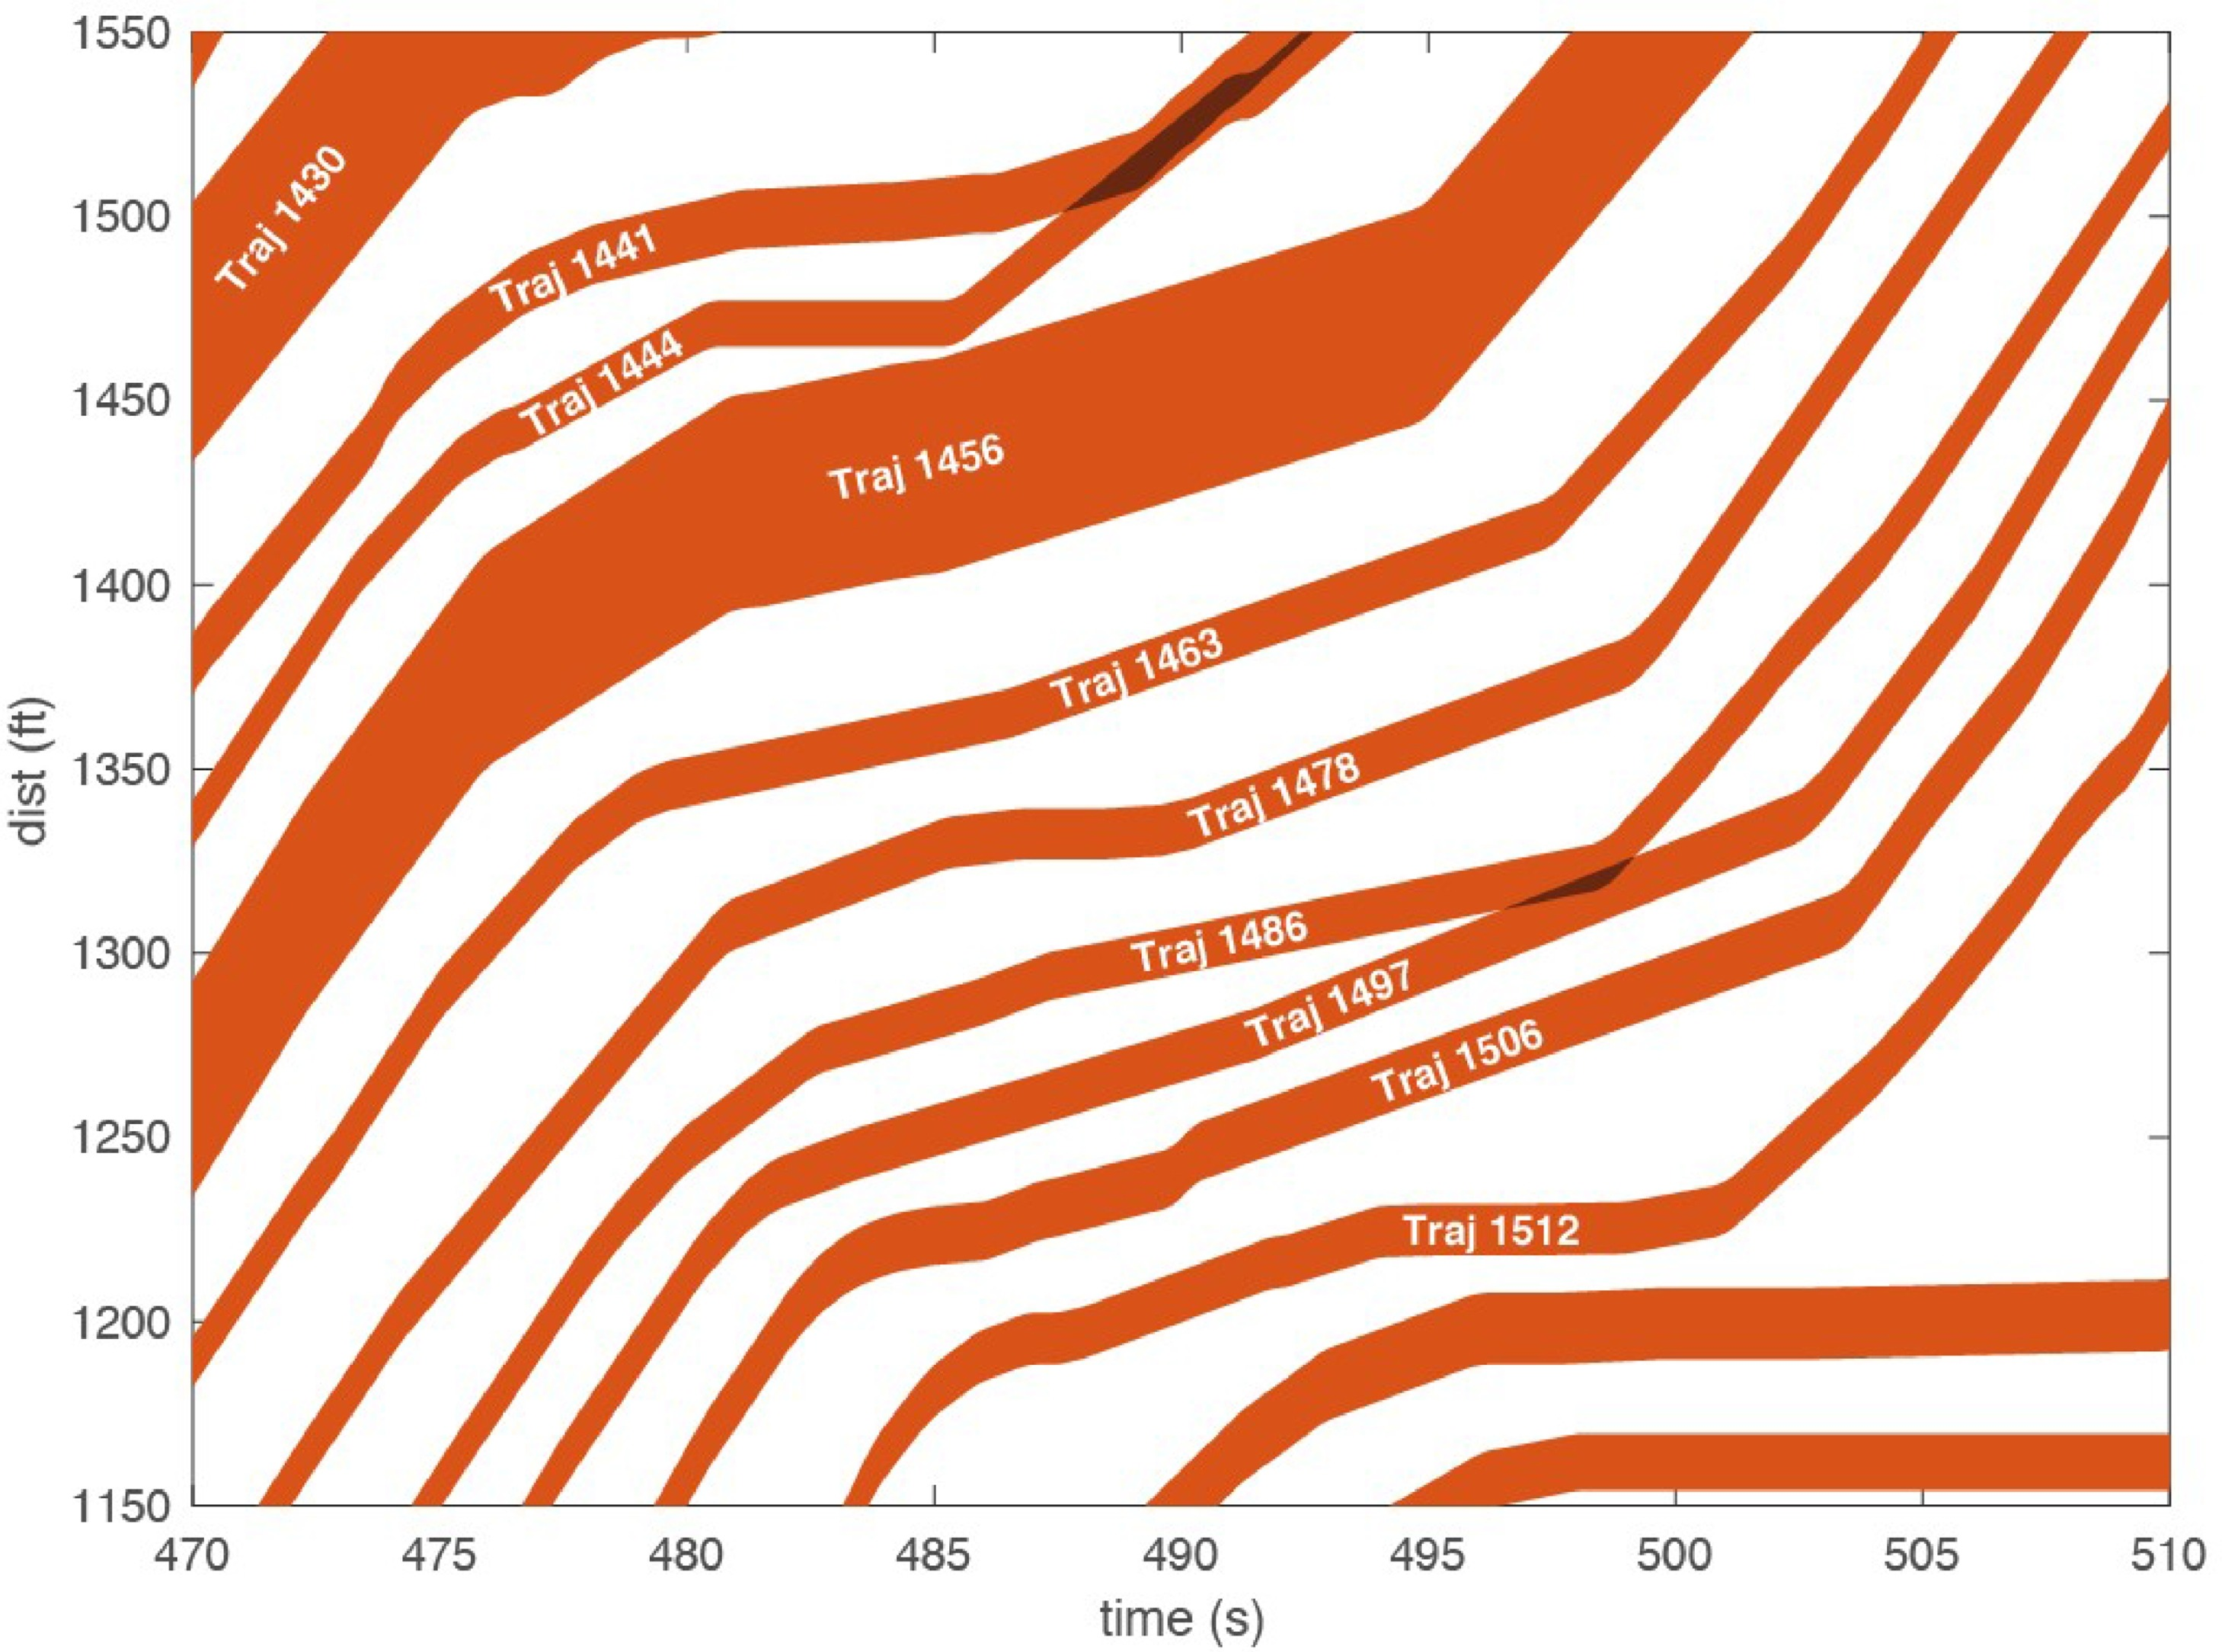
\includegraphics[]{{images/trajectorycollision.jpg}}
    \caption{\textit{Collisions of trajectories} errors. Orange areas are vehicles after taking their length into account. From Coifman and Li. \protect\cite{COIFMAN2017362}}
    \label{fig:collision}
\end{figure}

The first issue is that after accounting for vehicle length, trajectories often overrun those of proceeding vehicles seemingly resulting in \textit{collisions of trajectories}, first discovered by Thiemann et al. \cite{Thiemann_2008} The analysis of Coifman and Li. continues to address the second issue; Montanimo and Punzo \cite{MONTANINO201582} identified that the acceleration values in the dataset often exhibits unrealistically large magnitudes on the order of 10 $ft/s^2$ and likewise that the speed values exhibit unrealistic piecewise constant behaviour. In other words, some vehicles in the dataset maintain zero acceleration for an unrealistically long time, to the extent where it seems that the trajectories between two spatial points observed many seconds apart are estimated by performing linear interpolation during the NGSIM video image processing. %DOUBLE CHECK THE FIGURE NUMBER ONE LAST TIME

In order to alleviate the impact of these errors in the dataset to the model training, we discarded the particularly problematic acceleration attribute and performed sub-sectioning and time binning of the data, similar to the approach that Coifman and Li took to smooth the data, creating an image-like input for the model. To achieve that, the study section needed to be split into a number of sub-sections along the length of the highway. Therefore, we gave each datapoint an additional attribute, which is \textit{Distance} from the start of the section. The Euclidean distance was calculated simply taking the Local X and Local Y coordinates of the datapoint, since the section stretches almost straight. The section was then divided into 10 sub-sections, % NEEDS EDITS
each of which is roughly 200 feet in length. The distance attribute was then used to assign each datapoint to a sub-section, by adding the \textit{Section ID} attribute. In addition, the attributes deemed as unnecessary for the model training were also discarded; now the remaining attributes, which are \textit{Global Time}, \textit{Vehicle ID}, \textit{Lane ID}, \textit{Velocity}, and the newly added \textit{Distance} and \textit{Section ID}, continue to the further preprocessing.

\begin{figure}[ht!]
    \centering
    \includegraphics[width=10cm]{{images/output1.png}} % CHANGE THIS FIGURE
    \caption{Visualisation of average vehicle speed and density in each road section. At the start of their data collection, vehicles already in-frame are considered invalid observations. In our study, the values in the grid with these invalid observations were replaced with the default values of 60 mph for speed attribute and a zero value for density attribute.}
\label{fig:output1}
\end{figure}

Then, the datapoints were aggregated using the Section ID attribute, and now the data at each timestamp is binned into 10 sub-sections and the average speed and density of the vehicles in each sub-section at each timestamp is calculated. In the beginning of the traffic observation, some parts of the study section are not filled with datapoints yet as seen in Fig. \ref{fig:output1}, so we decided to discard the first 45 seconds of the data to remove such noise in the training data. Then, time series aggregation was performed to fill as many sub-sections as possible with non-zero density and speed values at each interval. We found that for this particular dataset the timewindow of 0.5 seconds is most favourable since the aggregated values cover all grids and creates as many samples as possible for training. If we aggregated by a longer time window, the values would lose some magnitude of temporal features. For real-time prediction, the timewindow of 0.5 seconds was too short due to limited computational resource, and thus we used the timewindow length of 10 seconds. In addition, we performed a further data manipulation in which we filled null values with appropriate and plausible values. For this study, zero values for density attribute and the maximum speed limit of 60 mph for speed attribute were used to reduce as much computation as possible, although the average speed of vehicles in the proceeding and following grids can also be used. 

To create the 3D tensors, the Spark dataframes containing \textit{Timewindow ID}, \textit{Section ID}, \textit{Lane ID}, \textit{Speed}, and \textit{Density} attributes were converted to RDDs, and the RDDs were grouped by key and then mapped to a key-value pair, where the key is the interval ID and the value is Row objects containing the speed and density values of each sub-section at each interval. The key-value pairs were then converted to a numpy array in a User Defined Function, and the returned numpy arrays were stacked to create the 4D tensor, with a shape of $R^{T{\times}M{\times}N{\times}L}$, where $T$, $M$, $N$, $L$ denotes the number of timewindows (intervals), the height of grid (lanes), the width of grid (sub-sections), the number of attributes, respectively. The main component of this operation is represented in Algorithm \ref{alg:rddto3d} in Appendix A. % include psuedo code?

Training a model to forecast the state of traffic of the future requires the past data as well as target data. Therefore, we have to provide another dimension to the tensor, creating a stack of 4D tensors of the fixed length of intervals, which results in a 5D tensor with a shape of $R^{s{\times}p{\times}M{\times}N{\times}L}$, where $s$, $p$, $M$, $N$, $L$ denotes the number of samples, the number of timewindows to look back or the prediction target timewindows, the height of grid (lanes), the width of grid (sub-sections), the number of attributes, respectively. Furthermore, in order to provide the model an extra time for inference, the prediction target data were offset by a fixed number of intervals, which is the \textit{skip} parameter. This operation was performed sliding the ``window" by the time series aggregation interval, and the resulting 5D tensor was then split into training and test datasets. This process is represented in Fig. \ref{fig:3dto5d} from a high-level perspective and explained in Algorithm \ref{alg:offset4d} in Appendix A from an implementation-level perspective. % include psuedo code?

\begin{figure}[ht!]
    \centering
    \includegraphics[width=14cm]{{images/3dto5d.png}}
    \caption{Gantt chart-like representation of the transformation of the data from 3D to 5D tensor. Firstly, 3D matrices are stacked to create a 4D tensor, and the fixed number of 4D tensors are stacked to create a stack of past data and target data. Then, they will be again stacked to create a batch, resulting in 5D tensor.}
    \label{fig:3dto5d}
\end{figure}

\section{Model}

The model used in this study is a Mixed Deep Learning (MDL) model, which consists of a sequence of deep learning layers which includes a Convolutional Neural Network (CNN) and a Convolutional long short term memory neural network (Conv-LSTM), which is a combination of a Convolutional Neural Network (CNN) and a Long Short-Term Memory (LSTM) network. The model was originally introduced by Lu et al. \cite{9284587} for the prediction of lane-level traffic speeds. For lane-level traffic state prediction, it is important to make the model capture the variable traffic state over time as well as behaviours of surrounding vehicles. The model is designed to effectively capture these spatial and temporal dependencies in vehicle trajectory data, and it has been shown to outperform other models such as the LSTM and the Conv-LSTM in terms of prediction accuracy. In this section, we first introduce the underlying ideas of MDL, which are the standard LSTM and the Conv-LSTM, then move on to the description of the Mixed Deep Learning model.

\subsection{Convolutional Long Short Term Memory Neural Network}
Conv-LSTM, which MDL is based on, is a type of neural network that combines the spatial processing capabilities of CNN with the temporal processing capabilities of an LSTM to handle spatio-temporal data. Conv-LSTM was first proposed by Shi et al \cite{convlstm}. In short, the idea is to add Convolutional operations to an LSTM cell. This section first introduces the LSTM, then extend it into Conv-LSTM.

Traditional Recurrent Neural Networks (RNNs) can track arbitrary long-term dependencies in sequential data. However, while training a traditional RNN, it performs backpropagation in which it updates the weights in the network by calculating the gradient of the loss function with respect to the weights. The problem is that the longer the input sequence is, the more vulnerable it becomes to the phenomenon called vanishing gradient problem, where the gradient of the loss function becomes too small to update the weights, causing the model training to slow down or possibly come to a complete halt. % DO I NEED TO ADD MATHEMATICAL FORMULA?

In order to address this issue, Long Short-Term Memory (LSTM) was introduced by Hochreiter and Schmidhuber \cite{lstm}. The comparison of RNN and LSTM structures is visualised in Fig. \ref{fig:rnnvslstm}. The key idea behind LSTM is the introduction of a memory cell in the hidden layer, which is a container of the cell state $c_t$ in which information gets stored over longer periods of time. The memory cell has three special structures that allow information to selectively influence the cell state at every moment: the input gate, the forget gate, and the output gate. The input gate $i_t$ controls the input of information to the memory cell, the forget gate $f_t$ controls the removal of information from the memory cell, and the output gate $o_t$ controls what information is output from the memory cell. The gates are controlled by sigmoid activation functions $\sigma$, which output values between 0 and 1, and a tanh activation function, which outputs values between -1 and 1. The gates are trained to learn which information to keep and which information to discard.

Let $T$, $x$, $h$ be the number of the timestamps, the input vector sequences, and the output vector sequences of the hidden layer, respectively, the structure of LSTM neural network can be written in the following equations:
\[t = 1, 2, ..., T\]
\[x = (x_{1}, x_{2},..., x_T)\]
\[h = (h_{1}, h_{2},..., h_T)\]
\[f_t = \sigma(w_{xf} x_t + w_{hf} h_{t-1} + w_{cf} \odot c_{t-1} + b_f )\]
\[i_t = \sigma(w_{xi} x_t + w_{hi} h_{t-1} + w_{ci} \odot c_{t-1} + b_i )\]
\[c_t = f_t \odot c_{t-1} + i_t \odot \tanh(w_{xc} x_t + w_{hc} h_{t-1} + b_c)\] 
\[o_t = \sigma(w_{xo} x_t + w_{ho} h_{t-1} + w_co \odot c_t + b_o)\]
\[h_t = o_t \odot \tanh(c_t)\]
where
$\odot$ denotes the Hadamard product (element-wise multiplication) of two vectors, matrices, or tensors with the same dimension;
$\sigma$ is the sigmoid activation function;
$w_{hi}$, $w_{hf}$, $w_{ho}$ and $w_{xi}$, $w_{xf}$, $w_{xo}$ are the weight matrices for the input, forget, and output gates, respectively;
$w_{ci}$, $w_{cf}$, $w_{co}$ are the weight matrices for the cell state;
$b_i$, $b_f$, $b_o$, $b_c$ are the bias terms for the input, forget, and output gates, and cell state, respectively.

\begin{figure}[ht!]
    \centering
    \subcaptionbox{\label{i3}}{
        \includegraphics[width=12cm]{images/rnn.png}
    }
    \subcaptionbox{\label{i4}}{
        \includegraphics[width=12cm]{images/lstm.png}
    }
\caption{The comparison between (a) RNN and (b) LSTM structures.}
\label{fig:rnnvslstm}
\end{figure}

The standard LSTM is suitable for 1D sequential data processing, and yet it is not capable of effectively capturing the contextual information of pixel data, thus it is not ideal for 2D and 3D signal processing tasks such as images and feature maps. Conv-LSTM extends the LSTM by adding convolutional operations to both the input-to-state and state-to-state transitions in the LSTM cell, which allows the model to learn spatial features as well as temporal features from the input data. The Conv-LSTM cell has the same structure as the LSTM cell, apart from the aforementioned modification to the LSTM cell. The mathematical equations of the Conv-LSTM cell are summarised as follows according to \cite{9779153}:
\[I_t = \sigma(W_{xi} * X_t + W_{hi} * H_{t-1} + W_{ci} \odot C_{t-1} + b_i)\]
\[F_t = \sigma(W_{xf} * X_t + W_{hf} * H_{t-1} + W_{cf} \odot C_{t-1} + b_f)\]
\[C_t = F_t \odot C_{t-1} + I_t \odot \tanh(W_{xc} * X_t + W_{hc} * H_{t-1} + b_c)\]
\[O_t = \sigma(W_{xo} * X_t + W_{ho} * H_{t-1} + W_{co} \odot C_t + b_o)\]
\[H_t = O_t \odot \tanh(C_t)\]
where $*$ denotes the convolution operator. Note that $X_t$, $C_t$, $H_t$, $I_t$, $F_t$, $O_t$ $\in$ $R^{M \times N \times L}$, where $R^{M \times N \times L}$ denotes the space of the 3D tensor, and $M$, $N$, and $L$ are the height, width, and each grid feature vector of the tensor, respectively. 

\begin{figure}[ht!]
    \centering
    \includegraphics[width=11cm]{{images/convlstm.png}}
    \caption{Inner structure of a ConvLSTM cell}
\end{figure}

In a Conv-LSTM layer, an input tensor $X = (X_1, X_2,..., X_T)$ is processed into an input tensor $H = (H_1, H_2,..., H_T)$, where $T$ refers to the number of the timestamps. Therefore, each Conv-LSTM layer can be described as a mapping function $F^{CL}: R^{T{\times}M{\times}N{\times}L} \rightarrow R^{T{\times}M{\times}N{\times}L^{\prime}}$, with $L$ representing the length of one input feature vector in each grid and $L^{\prime}$ indicating the length of the output feature vector in each grid. %PARAPHRASE THIS PARAGRAPH


\subsection{Mixed Deep Learning Model}

Mixed Deep Learning (MDL) model was proposed by by Lu et al. \cite{9284587} to forecast the traffic speeds of lane sections. The structure of the MDL model is shown in Fig. \ref{fig:mdl}. The model simplifies the study area of the road as $m{\times}n$ grids, where $m$ is the number of lanes and $n$ is the number of the road sections at one road section. Each grid represents the area of a road section and a $m{\times}n$ matrix stores values for a spatio-temporal variable such as traffic speed and vehicle density. Looking at the third to fifth dimensions of the aforementioned 5D tensor and taking each attribute (speed and vehicle density) from the aforementioned tensor, we can translate the third to fifth dimensions of the original tensor into a tensor of ${V_t}$ and ${D_t}$ with dimension of $M{\times}N{\times}1$, which contains each attribute variables during the time series aggregation interval $t$. The prediction target vector $Y_t$ contains traffic speed of all sections during the timewindow $T_h$ and length of the $Y_t$ is $T_h{\times}M{\times}N$, where $T_h$ is the forecast horizon with an offset of the skip parameter. % POSSIBLY MATHEMATICALLY INPRECISENESS

Since it is important to speed up training and inference time especially when real-time inference is in mind, we attempted to downsize the model as well as reduce the number of attributes to be fed into the architecture, which differs from the original MDL model. The original MDL architecture, where the two kinds of variables (historical travel speed and vehicle density) are fed into two separate architectures of stacked Conv-LSTM and CNN layers, was also tested for static prediction. Here, let $L_s$ and $L_q$ be the numbers of the stacked Conv-LSTM layers in the architectures for speed and vehicle density, the downsized model's $L_s$ is $1$, whereas the original model's $L_s$ and $L_q$ are $2$. Note that the downsized model has only one stream (architecture), as shown in Fig. \ref{fig:downsizedmdl}. $T_b$ represents the input historical timewindow of speed variable, and also vehicle density variable for the original MDL model. The architecture for the spatio-temporal variable for the speed attribute can be generalised and formulated as follows:
\[ (U^{L_s}_{t-T_b}, U^{L_s}_{t-T_b+1},..., U^{L_s}_{t-1}) = F^{CL}_{L_s}...F^{CL}_{l}...F^{CL}_{1} (V_{t-T_b}, V_{t-T_b+1},..., V_{t-1}) \]
\[ \hat{Y^s_{t}} = {\sigma}_r (W_s\ast{U^{L_s}_{t-1}} + b_s) \]
The original MDL model considers an additional spatio-temporal variable which is the vehicle density attribute, adding the following architecture to the model in parallel:
\[ (G^{L_q}_{t-T_b}, G^{L_q}_{t-T_b+1},...,G^{L_q}_{t-1}) = F^{CL}_{L_q}...F^{CL}_{l}...F^{CL}_{1} (D_{t-T_b}, D_{t-T_b+1},..., D_{t-1}) \]
\[ \hat{Y^q_{t}} = {\sigma}_r (W_q\ast{G^{L_q}_{t-1}} + b_q) \]
where $U^{L_s}_{t-t^{\prime}}$, $t\prime = 1, 2,..., T_b$ and $G^{L_q}_{t-t^{\prime}}$, $t\prime = 1, 2,..., T_b$ refer to output hidden tensors in the highest-level layers of the speed and volume, respectively; $W_s$ and $W_q$ denote the additional convolutional operators to augument the spatial correlation capturing of the high-dimensional output tensors from the Conv-LSTM layers; $b_s$ and $b_q$ are the bias tensors; $\sigma_r$ is the ReLU activation function.

During convolution process in the MDL model, the widely-used filter size of 3$\times$3 was also used for this study. In order to avoid the output feature map size reduction, often resulting in the loss of information on the edges of the input feature map, we also applied the zero-padding method in which it creates zero values around the input feature map before the process.

Then, we flatten the output obtained from the convolutional layers $\hat{Y^{s}_t}$, followed by feeding the vector to the fully connected layer. The original architecture has an additional operation after obtaining the two outputs $\hat{Y^{s}_t}$ and $\hat{Y^q_t}$: they are flattened and fused into one vector by performing concatenation:
\[ \hat{Y_t} = W_y \times Conc[F(\hat{Y^s_t}), F(\hat{Y^q_t})] + b_y\]
where $F(\cdot)$ is the flatten operation, $Conc(\cdot)$ is the concatenation operation, $W_y$ and $b_y$ are the weight and bias, respectively. % PUT PSUDOCODE

During the training, the model is trained to minimise the mean squared error between the predicted and the actual traffic speeds using the objective function:
\[\min_{W, b} \parallel \hat{Y_t} - Y_t \parallel^2_2 + \alpha \parallel W \parallel^2_2 \]
where $\hat{Y_t}$ and $Y_t$ are the predicted speed vector and the actual speed vector, respectively; $\alpha \parallel W \parallel^2_2$ is the L2-norm regularisation term to reduce overfitting; $W$ refers to the weighted parameters in $\hat{Y_t}$; $\alpha$ is a regularisation parameter.

The implementation of the MDL model is based on the authors' code\footnote{https://github.com/lwqs93/MDL} with modifications to suit it to our dataset and framework. Our code can be found on Github\footnote{}. % ADD THE LINK

\begin{figure}[ht!]
    \centering
    \includegraphics[width=14cm]{{images/MDL.png}}
    \caption{The structure of the orginal MDL model. From Lu et al. \protect\cite{9284587}}
    \label{fig:mdl}
\end{figure}

\begin{figure}[ht!]
    \centering
    \includegraphics[width=13cm]{{images/downsizedmdl.png}}
    \caption{The structure of the downsized MDL model used for real-time prediction. Note that the downsized model has only one stream of processing: speed, and thus no merging operation.}
    \label{fig:downsizedmdl}
\end{figure}

\clearpage
\section{Real-time Streaming Architecture}

\begin{figure}[ht!]
    \centering
    \includegraphics[width=14cm]{{images/realtime_arch.png}}
    \caption{The proposed architecture of real-time prediction data pipeline.}
    \label{fig:realtime_arch}
\end{figure}

In this section, we describe the architecture of the real-time prediction data pipeline. Fig. \ref{fig:realtime_arch} represents the architecture. % DOUBLE CHECK THE FIGURE NUMBER ONE LAST TIME
The pipeline consists of three main components: the data ingestion component, the Kafka streaming component, and the Spark Structured Streaming component.

In this study, we replicated an API by defining a function in which the 20 percent of the total datapoints reserved for testing are converted to JSON strings and ingested chunk by chunk to Kafka server every 0.1 second, which is the same as the original data collection interval. The chunk of datapoints stored in a Kafka topic are then streamed to the Spark Structured Streaming component, where the data is preprocessed and aggregated by the time series aggregation interval $t$, using \textit{watermarking}\footnote{Refer to the Apache Spark Structured Streaming documentation for further details: https://spark.apache.org/docs/latest/structured-streaming-programming-guide.html}. This operation allows Spark to further create a 3D matrix with dimension of $R^{M{\times}N{\times}L}$, which was already explained in Section \ref{data_preprocessing}, but in a streaming fashion. Note that since Spark Strcutured Streaming does not support RDD conversion, the matrix creation is performed within the Spark DataFrame API, without converting to RDDs, which is a key difference from the preprocessing process of creating the training input data. 

After parsing the dataframe to JSON string, the data stream is again ingested to the Kafka server, but into a different Kafka topic. The data is then streamed to the Spark Structured Streaming component, where this time the dataframe is aggregated by the length of historical timewindow $T_b$. The reason for rewriting the data back to a Kafka topic is that Spark Structured Streaming is yet to support double watermark aggregations within a single Spark context. Now the dataframe contains a 4D tensor with dimension of $R^{T{\times}M{\times}N{\times}L}$ within a column. The tensor is converted to a numpy array and fed into the trained model in a User Defined Function (UDF) registered in each Spark DataFrame Row. After the UDF stores predicted speed values in a new column, the JSON string parsed from a dataframe is streamed to the Kafka server, where the predicted speed values are stored in another Kafka topic. The predicted speed values can be then visualised in real-time using a dashboard or used for various applications such as Advanced Driver-Assistance Systems (ADAS) and Autonomous Vehicles (AVs). 

\section{Evaluation Method}

According to the literature survey of Li et al. \cite{li2024unifyinglaneleveltrafficprediction}, the lane-level traffic prediction model accuracy is evaluated typically using three key metrics: Mean Absolute Error (MAE), and Mean Absolute Percentage Error (MAPE), Root Mean Squared Error (RMSE). However, the researchers also emphasise the importance of considering the duration of its training when the model is to be used in real-time lane-level traffic prediction, where rapid response and real-time updates are essential. This paper also puts an emphasis on the architecture of real-time inference, and thus instead of considering the training time, the time taken for inference as well as data preprocessing within the streaming architecture is evaluated. The formulas for the three metrics are as follows:
\[ MAE = \frac{1}{n}\sum_{i=1}^{n}|\hat{Y_i} - Y_i| \]
\[ MAPE = \frac{1}{n}\sum_{i=1}^{n}\frac{|\hat{Y_i} - Y_i|}{Y_i} \times 100\% \]
\[ RMSE = \sqrt{\frac{1}{n}\sum_{i=1}^{n}(\hat{Y_i} - Y_i)^2} \]
\[ Inference Time = \frac{1}{n}\sum_{i=1}^{n}t_i \]
where $\hat{Y_i}$ is the predicted speed, $Y_i$ is the actual speed during $i$-th time interval, $n$ is the total number of predicted samples, and $t_i$ is the preprocessing and inference time of the $i$th sample.

However, there is one significant limitation of MAPE that is the metric can produce very high or even close to infinity values especially when the values to be evaluated contain zeros or values close to zeros. Since the scale of actual values in the dataset is relatively in a small range of 0 to 60 mph, the MAPE metric is not particularly suitable for the evaluation of the model. Therefore, we calculated the Mean Arctangent Absolute Percentage Error (MAAPE) in addition to the three error ratio matrics mentioned above. The MAAPE metric was introduced by Kim et al. \cite{KIM2016669} as a more robust alternative to MAPE, which considers the error ratio as an angle instead of a slope unlike MAPE and is less sensitive to the scale of the actual values. The formula for MAAPE is as follows:
\[ MAAPE = \frac{1}{n}\sum_{i=1}^{n} \arctan\left(\frac{|\hat{Y_i} - Y_i|}{Y_i}\right) \times 100\% \]

% MAYBE ELABORATE MORE ON MAAPE

% Difference in Accuracy between the original and downsized model -> does downsizing the model affect the accuracy?
% Difference in Accuracy between different timewindow lengths and number of lanes considered -> does the aggregation window length and the number of lanes considered affect the accuracy?
% Difference in Accuracy between static and real-time prediction -> does the streaming architecture and datapoint loss affect the accuracy?
% Inference time of the real-time prediction -> how long does it take to predict the traffic speed in real-time? and how long should the skip parameter be set to to achieve real-time inference?
% Difference in Accuracy between different skip parameters in real-time prediction -> does the skip parameter affect the accuracy?
In the experiments, we evaluated the two models from the four different perspectives with the following objectives:
\begin{itemize}
    \item Difference in accuracy between the original MDL model and the downsized version of the model, to check if downsizing the model affects the accuracy.
    \item Difference in accuracy of the models with different data preprocessing parameters such as the time series aggregation window length, the number of lanes considered, and the skip parameter, to investigate how the aggregation window length, inclusion of on- and off-ramp in the input data, and the length of a target timewindow offset affect the accuracy.
    \item Difference in accuracy of the downsized models in different prediction modes: non-real-time and real-time prediction, considering the impact of datapoint losses during streaming on accuracy.
    \item Inference time of real-time predictions, to prove the feasibility of real-time prediction and to determine how long the skip parameter should be set to achieve real-time inference.
\end{itemize}

Table \ref{Tab:models} summarises all models evaluated in this study. Non-real-time (Static) prediction models are evaluated using 20 percent of the total datapoints reserved for testing, comparing the predicted values and the ground truth values all at once at the end of model training. Real-time prediction model and the architecture are evaluated using the streaming architecture described in the previous section; a small chunk of datapoints from the reserved 20 percent test data was ingested to the Kafka server every 0.1 second, and we collected the predicted values from the Kafka server and compared the predicted values with the ground truth values at the end of the streaming. The inference time was calculated by measuring the total time from the time when the last chunk of data of the first sample was ingested to the Kafka server to the time when the model produced the predicted values of the last sample, and then dividing the total time by the number of samples obtained.

\begin{table}[ht!]
    \centering
    \begin{tabular}{ |P{3cm}|P{2.5cm}|P{2cm}|P{2cm}|P{2cm}|P{1.5cm}| }
        \hline
        Models & Input Feature & Conv-LSTM layers number & Timewindow & On-Off Ramp Included & Skip \\
        \hline
        \multirow{4}{*}{\shortstack[1]{Original MDL\\(Static)}} & \multirow{4}{*}{speed, density} & \multirow{4}{*}{2} & 0.5 sec & Yes & 10 sec\\
         & & & 0.5 sec & No & 10 sec\\
         & & & 10 sec & Yes & 10 sec\\
         & & & 10 sec & No & 10 sec\\
        \hline
        \multirow{4}{*}{\shortstack[1]{Downsized MDL\\(Static)}} & \multirow{4}{*}{speed} & \multirow{4}{*}{1} & 0.5 sec & Yes & 10 sec\\
         & & & 0.5 sec & No & 10 sec\\
         & & & 10 sec & Yes & 10 sec\\
         & & & 10 sec & No & 10 sec\\ 
        \hline
        \multirow{2}{*}{\shortstack[1]{Downsized MDL\\(Real-time)}} & \multirow{2}{*}{speed} & \multirow{2}{*}{1} & 10 sec & No & 10 sec\\
        & & & 10 sec & No & 20 sec\\
        \hline
    \end{tabular}
\caption{List of evaluated models\label{Tab:models}}
\end{table}


\chapter{Results and Discussion}

All experiments were conducted on a computer with an Intel Core i5 Quad-Core CPU at 2.3GHz and 16GB of RAM. No GPU is used in this study. The training and evaluation were performed using PySpark 3.5.1, Kafka 3.8.0, Keras 3.4.1 and TensorFlow 2.16.2 as its backend. The models were trained using the Adamax optimiser with a learning rate of 0.001, and the batch size was set to 16. The models have 3 filters in each ConvLSTM layer's convolution and 1 filter in the convolutional layer. Each model was trained for 50 epochs with the early stopping engaged. 

% ORGANISE THE RESULTS: 1) Original vs downsized accuracy, 2) static and realtime (both accuracy and inference time), 3) different time window etc parameters

\section{Original vs Downsized Models}
The results for accuracy are shown in \ref{Tab:originalvsdownsized}. % DOUBLE CHECK THE TABLE NUMBER ONE LAST TIME

\begin{table}[ht!]
    \centering
    \begin{tabular}{ |c|c|c|c|c|c|c| }
        \hline
        Model & Timewindow & On-Off Ramp Included & MAE & MAPE & MAAPE & RMSE\\
        \hline
        \multirow[vpos]{4}{*}{Original} & 0.5 sec & Yes & 8.28 & $\infty$ & 35.19\% & 13.16\\
        & 0.5 sec & No & 9.63 & $\infty$ & 41.32\% & 15.31\\
        & 10 sec & Yes & 7.10 & \textbf{58.67\%} & \textbf{34.23\%} & 10.90\\
        & 10 sec & No & 7.40 & 65.22\% & 37.91\% & 11.42\\
        \hline
        \multirow[vpos]{4}{*}{Downsized} & 0.5 sec & Yes & 8.62 & $\infty$ & 36.52\% & 13.54\\
        & 0.5 sec & No & 8.87 & $\infty$ & 40.25\% & 13.69\\
        & 10 sec & Yes & 7.21 & 60.67\% & 35.07\% & 10.66\\
        & 10 sec & No & \textbf{7.06} & 64.42\% & 36.99\% & \textbf{10.51}\\
        \hline
    \end{tabular}
\caption{Results of original and downsized MDL models evaluated for static prediction. The best result of each category is highlighted in bold.\label{Tab:originalvsdownsized}}
\end{table}

% Effect of the downsizing of the model on accuracy
In Table 4.1, we can see that in terms of accuracy there was no significant difference between the original MDL model and the downsized MDL overall. The downsized model is computationally less expensive than the original model, which makes it more suitable for real-time prediction.

\begin{figure}[ht!]
    \centering
    \includegraphics[width=10cm]{{images/mdl_res_comp.png}}
    \caption{Comparison between the actual and predicted speed values of the downsized MDL model with the timewindow of 10 sec and the on- and off-ramp sections included}
    \label{fig:mdl_model_w_10_10_6_1_1_velocity_output_2299.5}
\end{figure}

% Effect of including on- and off-ramp sections on accuracy
On the subject of comparison between the accuracy of the models with the on- and off-ramp sections included and the models without them, we can see that the model that considers them performs better than the model that does not. This could be due to one of the data preprocessing steps introduced to this study to make the matrix data learnable for the model. Since the vehicles travelling on the on- and off-ramp between the section 0-1 and the section 6-9 are not recorded in the dataset, we filled the grids with a null value with a constant value of 60 mph to make the matrix data learnable for the model. As we can see in Fig. \ref{fig:mdl_model_w_10_10_6_1_1_velocity_output_2299.5}, % CHECK THE FIGURE NUMBER ONE LAST TIME
the error ratio of those grids is lower than the that of the other grids. The greater number of grids with a slim difference between the actual and predicted speed values results in better prediction accuracy.

% Effect of the length of the timewindow on accuracy
Also, the models with the longer length of time series aggregation window perform better than those with the shorter length. During the data preprocessing, we averaged aggregated values of the speed and density, which could mean the longer timewindow length resulted in the reduced intensity of the temporal features. The fewer number of outliers and the smaller range of values in the data could have made the model learn the data more effectively and thus predict the future state of the traffic more accurately. However, we have to consider the trade-off between the model accuracy and the timewindow length and how much extension of the timewindow length a real-world application of the model can tolerate, as the longer timewindow length makes the model less real-time and less sensitive to granularity of the traffic state.

\section{Real-time Prediction}

\begin{table}[ht!]
    \centering
    \begin{tabular}{ |c|c|c|c|c|c|c|c| }
        \hline
        Mode & Timewindow & Skip & MAE & MAPE & MAAPE & RMSE & Inference Time\\
        \hline
        Static & 10 sec & 10 sec & 7.06 & 64.42\% & 36.99\% & 10.51 & N/A \\ 
        \hline
        \multirow[vpos]{2}{*}{Real-Time} & 10 sec & 10 sec & 9.21 & $\infty$ & 45.07\% & 13.42 & 12.02 sec\\
        & 10 sec & 20 sec & 8.72 & $\infty$ & 44.13\% & 12.77 & 12.43 sec\\
        \hline
    \end{tabular}
\caption{Comparison between the accuracy of donwsized models with different skip parameters in different prediction mode.\label{Tab:realtime}}
\end{table}

% Comparison between the static and real-time prediction
Comparing the accuracy of the results produced from the static and the real-time prediction, we can see that real-time prediction with skip parameter of 10 seconds performs worse than the static prediction by 8\% in terms of MAAPE. This is due to the architectural design of handling the late arrival of the preprocessed data to the model within the proposed framework. Each chunk of historical data has to be in a complete shape before it is fed into the model, which means the model has to wait for the data to arrive to perform prediction. In order to remove this latency affecting the streaming, we decided to make the system escape the datapoints that are not in a complete shape at the time of prediction by returning zero values, which is effectively the loss of datapoints. Over the course of the studied time, we received 6 lost datapoints out of the total number of received datapoints of 47 for real-time prediction with 10 seconds skipping. For the 20 seconds skipping result, the accuracy was better than that of 10 seconds skipping due to its fewer lost datapoints, which was 4 out of 46, than what we observed in 10 seconds skipping. Although a longer skipping time, which means that the model predicts the traffic state of more distant future, generally lead to poorer accuracy, this unexpected result shows that the impact of the number of lost datapoints on accuracy outweighs that of a longer skipping time in our current architecture. We can also derive the phenomenon of data loss from the infinite MAPE of real-time model in Table \ref{Tab:realtime}. % DOUBLE CHECK THE TABLE NUMBER ONE LAST TIME

In terms of the experiments of real-time datapreprocessing and inference time, the total time length of studied data is 543.0 seconds and we collected the total number of samples of 47 for the real-time prediction experiment. The total inference time of the studied data was 564.84 seconds, and therefore the average data preprocessing and inference time per sample was 12.02 seconds. The skip parameter was set to 10 seconds, which means the real-time inference was lagging by 2.02 seconds per sample on average. This result indicates that the current data pipeline with skip paramter of 10 seconds cannot handle the prediction in real-time. However, by extending the skip parameter to 20 seconds, the real-time prediction was able to achieve the average inference time of 12.43 seconds per sample, which means the model was able to predict the traffic state of 7.57 seconds ahead of the current time. The result shows that the current architecture is neither satisfactory nor stable enough, yet it is still capable of predicting the traffic state in real-time under certain conditions. % MAYBE TRY MULTIPLE TIMES AND TAKE THE AVERAGE?

In summary, the key findings in the experiments are: (1) the downsized model is as accurate as the original model, and thus it can be considered more suitable for real-time prediction; (2) the models with the on- and off-ramp sections included performs better than those without them; (3) the models with the longer timewindow length perform better than those with the shorter timewindow length; (4) the real-time prediction model with the skip parameter of 20 seconds is more accurate than the model with the skip parameter of 10 seconds; (5) and the particular model is capable of predicting the traffic state of 7.57 seconds ahead in real-time.

\chapter{Limitations and Future Work}
% Reflection on the paper with the initial objectives, etc. (refer to the student handbook)
% mention that the dataset's quality limitation and lack of smoothing of the data: use lane1speeddist.png
% Mention that time series aggregation window length has to be further optimised by feature correlation analysis method
% Mention that the limitation of euclid calculation of distance from origin on bends or curves
% Mention that the model can be further optimised by hyperparameter tuning
% Mention that the model does not consider the impact of weather conditions or road condition anomalies
% mention that the model training is not considered in the real-time prediction architecture
% Mention that the model does not consider the impact of the vehicle type
% Mention that the architecture is not tested in remote cloud environment and the impact of the network latency is not considered
% mention that more sophiticated handling of loss of datapoints during streaming is required
% lack of further scalability testing of the architecture
% instead of predicting the precise speed, we can do thresholding to predict the traffic state (congested, normal flow, etc.)

\section{Further Data Preprocessing}

In Chapter 3, we briefly explained about the quality of the dataset and how we addressed the issue in this study by aggregating data and not using the acceleration feature. Still, acceleration is an important indicator of the start of congestions and the end of them, and thus the model accuracy can improve by adding the feature to the model. However, as Coifman and Li \cite{COIFMAN2017362} showed that correcting acceleration feature in the dataset is possible not by strictly though data cleaning and interpolation, but only by making a laudable effort comparing the original video data with the dataset and manually extracting the longitudinal vehicle trajectories by calculating speed and acceleration of all non-motorcycle vehicles on every lane, we had to assume that such a task is beyond the scope of this study. Yet, this work can still incorporate more thorough data cleaning and feature engineering process, which can be a future work.

In this study, we assumed that the historical data length of 60 seconds and the target data length of 10 seconds is most likely optimal and exhibit most correlation of features between them from the shockwave pattern seen in Fig. \ref{fig:lane1}. % DOUBLE CHECK THE FIGURE NUMBER ONE LAST TIME
However, the set lengths are nor optimal or universal, and thus to make the model more accurate and robust to various road environment, the time series aggregation window length and the historical and target data length can be further optimised by a feature correlation analysis method as Li et al. \cite{9284587} suggest. The feature correlation analysis method applied in their study is based on the maximum information coefficient (MIC), which is capable of identifying a wide range of relationships between variables \cite{mic}. % IF POSIIBLE, ELABORATE MORE ON MIC AND ITS APPILCATION
Intuitively, MIC is the maximum mutual information between random variables $x$ and $y$ normalised by the minimum value of their joint entropy. However, as the calculation of MIC is computationally expensive as it involves the calculation of the joint entropy of the variables. According to the Shao and Liu \cite{miccomplexity}, the time complexity of the MIC calculation is $O(n^{2.4})$ when MIC parameters are default and they conclude that the application of MIC to big data analysis leads to long computation time. For real-time prediction, this extra computational time can be critical, and thus the development of new fast algorithm for MIC and overall more efficient feature correlation analysis methods is required to make the traffic state prediction model more accurate and robust to various road environments.

Also, the use of the Euclidean distance calculation from the origin of the road section to the target road section is not suitable for the road sections with bends or curves, and it hinders the model's robustness to different shapes of roads. The Euclidean distance calculation is based on the assumption that the road sections are linearly stretched. To improve the method of obtaining the distance feature, we either have to make vehicles collect the information of the distance travelled on the road by introducing road-side milepost sensors, or calculate distance between the target vehicle and the following vehicles in the same lane each by each, and chain the distances to obtain the total distance from the origin of the road section, so that it accounts for different shapes of roads.

\section{Further Model Optimisation}

As this paper focuses on the architecture of real-time inference, a minimum amount of effort was made to undertake hyperparameter tuning and optimisation of accuracy. The paper in which MDL model was first introduced by Lu et al. \cite{9284587} has shown the model accuracy reached MAE of 6.14, RMSE of 8.03, and MAPE of 12.26\%. However, the data used for their study is Beijing Municipal Commission of Transport and the data is collected by road sensors with the updating frequency of 2 minutes, which is different from the data used in this study. As we explained in Fig. \ref{data_preprocessing}, a longer timewindow length in theory results in the reduced intensity and the fewer number of outliers and the smaller range of values of temporal features, which makes the model learn the data more accurately. The researchers set the input time window for feature variables as 15, which is more than twice as long as the timewindow used in this study. We can attribute the difference in accuracy to the difference in the data and the length of historical timewindow. Nevertheless, there is still room for improvement in the model accuracy by further exploring different hyperparameters and optimisation of the model architecture.

External factors such as weather and road condition anomalies affect travel demand and road capacity significantly \cite{WANG2023107044}, and yet the model does not consider the impact of such factors. To our knowledge, there is no empirical vehicle trajectory open dataset which includes different weather and road conditions. However, training the model with the dataset that includes such features is essential for the model to be used in real-world applications. The collection of such data can be challenging since the chance of encountering of extreme conditions during a data collection period is low, and depending on weather condition and visibility, video calibration and data extraction can be difficult and consequently the data quality can deteriorate. However, with the development and wider prevalence of Autonomous Vehicles (AVs), the collection of such data is becoming more feasible than ever. With the introduction of more extensive and various types of data, the model can be more accurate and robust to various real-world road environments. 

\section{Further Architectural Optimisation and Scalability Testing}

As well as model optimisation, there is still room for improvement of the architectural design of real-time prediction. The framework only considers real-time prediction and does not consider the real-time model training. Although each section generally has distinct characteristics of traffic congestion patterns due to road structure and terrain, training the model in real time to make it adapt to ever-changing traffic state is also an important task to improve the model. Because of the introduction of the skip parameters, we could not design the architecture to enable the data preprocessing pipeline to perform time-series data indexing for the model training and real-time inference simultaneously. In addition, the architecture has to perform data processing in real-time and cannot afford any extra latency, which raises the bar for the implementation of real-time model training.

Similarly, the more sophisticated handling of late arrival of data and loss of datapoints during streaming is required. The current architecture simply returns zero values for the datapoints that are not in a complete shape at the time of prediction, which is effectively the loss of datapoints. The loss of datapoints can be critical for the model accuracy, and thus the architecture has to be designed to handle the late arrival of data more effectively, reducing as much latency as possible.

Also, We must note another major limitations of this study; the model and the evaluation of the real-time inference does not take network latency into account. The architecture was tested only on a local machine, and the impact of the network latency to the real-time inference time is not considered. In real-world applications, the model will be deployed on a remote cloud environment, and the latency of network communication between the data ingestion component, the Kafka streaming component, and the Spark Structured Streaming component can be a critical factor affecting the real-time inference time. The architecture has to be tested in a remote cloud environment to evaluate the impact of the network latency on the real-time inference time, which can be a future work.

Furthermore, due to the availability of data and the computational resources, the scalability of the architecture was not satisfactorily explored. The architecture has to be tested on multiple clusters and with a larger number of datapoints to evaluate the scalability of the architecture, to ensure real-world applicability of this framework.

\chapter{Conclusion}

In this study, we proposed a real-time streaming architecture for lane-level traffic speed prediction using the Mixed Deep Learning (MDL) model. From the literature, we first explored multiple traffic flow datasets and different types of prediction models in terms of their applicability to this study by clearly stating their advantages and disadvantages. Secondly, by exploiting the appropriate dataset (NGSIM dataset), tools (Apache Kafka and Spark) and models (MDL), we proposed the data preprocessing methods, model architecture, and the real-time prediction framework, and the experiments of the models. Thirdly, we evaluated the accuracy of each model and the inference time of the real-time prediction models. The notable findings were: (1) the model with the longer length of time series aggregation window and the model that considers the on- and off-ramp sections perform better than the other models; (2) The downsized MDL model performs as well as the original MDL model; (3) the real-time prediction model with the skip parameter of 20 seconds performs better than the model with the skip parameter of 10 seconds; (4) The real-time prediction model with the skip parameter of 20 seconds is able to predict the traffic state of 7.57 seconds ahead of the current time, and the average inference time per sample is 12.43 seconds. From these findings, we conclude that the proposed framework is capable of predicting the traffic state in real-time under certain conditions.

As we discussed in Chapter 5, there is still room for improvement in data preprocessing and the accuracy and robustness of the model: by conducting more thorough data cleaning and feature engineering, introducing an effective feature correlation analysis method and non-Euclidean distance calculation method, hyperparameter tuning, and including of additional dependencies such as weather and road condition anomalies. In addition, the limitation of the real-time prediction architecture lies in handling the late arrival of data and loss of datapoints during streaming, and the lack of scalability testing on clustered remote environment with a larger number of datapoints.

Despite incompleteness of the proposed model and architecture, we believe that the initial objectives of this study were largely covered, and we hope that the proposed framework will be another stepping stone to the further development of real-time lane-level traffic flow prediction models. As stated in the introduction, lane-level traffic flow prediction is growing its importance in IVICS for improving road capacity, reducing traffic congestion, and overall making it safer and more comfortable to drive on highways. We hope that this study will contribute to advancing real-time lane-level traffic flow prediction, and more generally, to the wider society.

% JUSTIFICATION: Scalability, implementation (Spark is more widely adopted and more mature than other frameworks like Flink)

%%%%%%%%%%%%%%%%%%%%%%%%%%%%%%%%%%%%%%%%%%%%%%%%%%%%%%%%%%%%%%%%%%%%%%%%%%%%%%%%%%%%m
\bibliography{refs.bib}
%\printbibliography

%%%%%%%%%%%%%%%%%%%%%%%%%%%%%%%%%%%%%%%%%%%%%%%%%%%%%%%%%%%%%%%%%%%%%%%%%%%%%%%%%%%%
\begin{appendices}

\chapter{Supplementary Materials I}

This section contains the pseudo-code and the visualisation of the operation for tensor creation for the training data.

\begin{algorithm}
    \caption{Algorithm to convert a RDD to a 3D Tensor}
    \label{alg:rddto3d}
    \begin{algorithmic}[1]
    \State $k$: a key to the RDD iterator
    \State $I$: a RDD iterable
    \State $M$: number of lanes
    \State $N$: number of sections

        \Procedure{Create3DTensor}{$key$, $I$, $M$, $N$}
        \State Create $m \times n$ matrix $V$ filled with 60 
        \State Create $m \times n$ matrix $D$ filled with 0
    
        \For{each Row object $r$ in Iterable $I$} 
            \State $m$ $\gets$ $r$[`lane']
            \State $n$ $\gets$ $r$[`section']
            \State $V$[$m$][$n$] $\gets$ $r$[`velocity']
            \State $D$[$m$][$n$] $\gets$ $r$[`velocity']
        \EndFor
        \State $R$ $\gets$ stack $V$, $D$ appending each element of $V$, $D$ along the third dimension
        \State \textbf{return} ($key$, $R$)
        \EndProcedure
    \end{algorithmic}
\end{algorithm}

\begin{algorithm}
    \caption{Algorithm to a 5D input tensor offsetting with skip parameter}
    \label{alg:offset4d}
    \begin{algorithmic}[1]
    \State $R$: 4D tensor with dimension of $R^{T{\times}M{\times}N{\times}L}$
    \State $h$: historical timewindow length
    \State $p$: prediction timewindow length
    \State $l$: skip parameter

        \Procedure{CreateOffsetTensors}{$R$, $h$, $p$, $l$}
        \State ($L_h$, $L_p$) $\gets$ (empty list, empty list) 
    
        \For{$i$ in range($h+l+p$ to $T$)} \Comment $T$ is the number of timewindows
            \State $L_h$[$i$] $\gets$ a slice of $R$: $R$[$i-h-l-p:i-l-p$] across all 4 dimensions
            \State $L_p$[$i$] $\gets$ a slice of $R$: $R$[$i-p:i$] across all 4 dimensions
        \EndFor \Comment $L_h$ and $L_p$ are now lists, each of whose elements are $s$ number of 3D tensor samples
        \State $\hat{R}$ $\gets$ Stack each set of 3D tensor samples from $L_h$, $L_p$ along the first dimension \Comment $\hat{R}$ is now a 5D tensor with dimension of $R^{s{\times}p{\times}M{\times}N{\times}L}$
        \State \textbf{return} $\hat{R}$
        \EndProcedure
    \end{algorithmic}
\end{algorithm}

\begin{figure}[ht!]
    \centering
    \subcaptionbox{}{
        \includegraphics[width=14cm]{images/alg2forloop.png}
    }
    \subcaptionbox{}{
        \includegraphics[width=11cm]{images/alg2after.png}
    }
\caption{The visualisation of the Algorithm 2. (a) The first two iterations of the for-loop. (b) The operation at Line 11.}
\label{fig:alg2}
\end{figure}
    
\end{appendices}

\end{document}